\section{The Promise and Challenges of Medical Devices}
Medical devices play an essential role in the care of patients around the world, and can have a life-saving effect.
To cite one example, 
an estimated 3 million people worldwide have implanted pacemakers (a heart rate adjustment device), with $\sim$600,000 added annually.
%Cardiac Pacemakers From the Patient's Perspective circ.ahajournals.org/content/105/18/2136.full
In the United States, 800,000 people have an implanted defibrillator (another heart rhythm management device), with 10,000 added monthly.
%http://asktheicd.com/tile/106/english-implantable-cardioverter-defibrillator-icd/how-many-people-have-icds/
Clinical trials have presented evidence that patients implanted with defibrillators have a mortality rate reduced by up to 31\%.

% MADIT II trial
The medical device is a \$289 billion market with \$110 billion within the US.
%Of that, , with this number projected to reach \$133 billion in 2016.
%http://selectusa.commerce.gov/industry-snapshots/medical-device-industry-united-states
Examples include everything from adhesive bandages to drug infusion pumps, surgical robots, deep brain stimulation systems and physiological closed-loop control systems like the artificial pancreas~\cite{pancreas_paul} which are in development.
%In fact, many device companies are in the no-revenue startup phase, indicating a vigorous research environment.
These are safety-critical technologies combining hardware and software, each of which must be rigorously verified to be efficacious and safe.

According to the US Food and Drug Administration, in 1996, 10\% of all medical device recalls were caused by software-related issues. 
This percentage rose to an average of 15\% of recalls from 2008 to 2012. Implanted cardiac pacemakers and defibrillators have approximately 80,000-100,000 lines of software code~\cite{pauljones} which essentially makes all sensing, control and actuation decisions autonomously within the human body, over the 5-7 year device lifetime. The primary challenge of high-confidence medical device software is to guarantee the device will never drive the patient into an unsafe condition even though we do not have complete understanding of the physiological plant. 
%The medical device market is worth \$289 billion.
%Of that, \$110 billion is in the US alone, with this number projected to reach \$133 billion in 2016.
%%http://selectusa.commerce.gov/industry-snapshots/medical-device-industry-united-states
%Examples include everything from adhesive bandages to surgical robots, including pacemakers (a heartbeat adjustment device) and devices still undergoing basic research like the artificial pancreas.
%In fact, many device companies are in the no-revenue startup phase, indicating a vigorous research environment.
%To take one example of the societal impact of medical devices, 
%an estimated 3 million people worldwide have implanted pacemakers, with an extra 600,000 added annually.
%%Cardiac Pacemakers From the Patient's Perspective circ.ahajournals.org/content/105/18/2136.full
%Clinical trials have presented evidence that patients implanted with defibrillators (another heart rate adjustment device) have a mortality rate reduced by up to 31\%.
%% MADIT II trial
%These are life-saving technologies combining hardware and software, each of which must be rigorously verified to be efficacious and safe.
%According to the US Food and Drug Administration, in 1996, 10\% of all medical device recalls were caused by software-related issues. 
%This percentage rose to an average of 15\% of recalls from 2008 to 2012. 

\subsection{Human-in-the-loop Medical Devices}
Medical devices can be classified as open-loop or closed-loop.
A \emph{closed-loop device} like a pacemaker is in a feedback loop with the organ(s) it affects (see Fig.\ref{fig:pacemaker}): it monitors certain physiological variables like heart rate, and delivers therapy, in the form of low-energy electrical pulses, to maintain a healthy heart rate.
Another example is the artificial pancreas, which monitors blood glucose levels and delivers therapy, in the form of insulin, to maintain safe glucose levels.
An \emph{open loop device} on the other hand, either, (a) like a drug infusion pump, does not measure any physiological variables: the therapy it delivers is pre-programmed and non-reactive; or (b) as in the case of a blood pressure monitor, only measures physiological signals but does not deliver therapy. 
\begin{figure}[t]
	\centering
	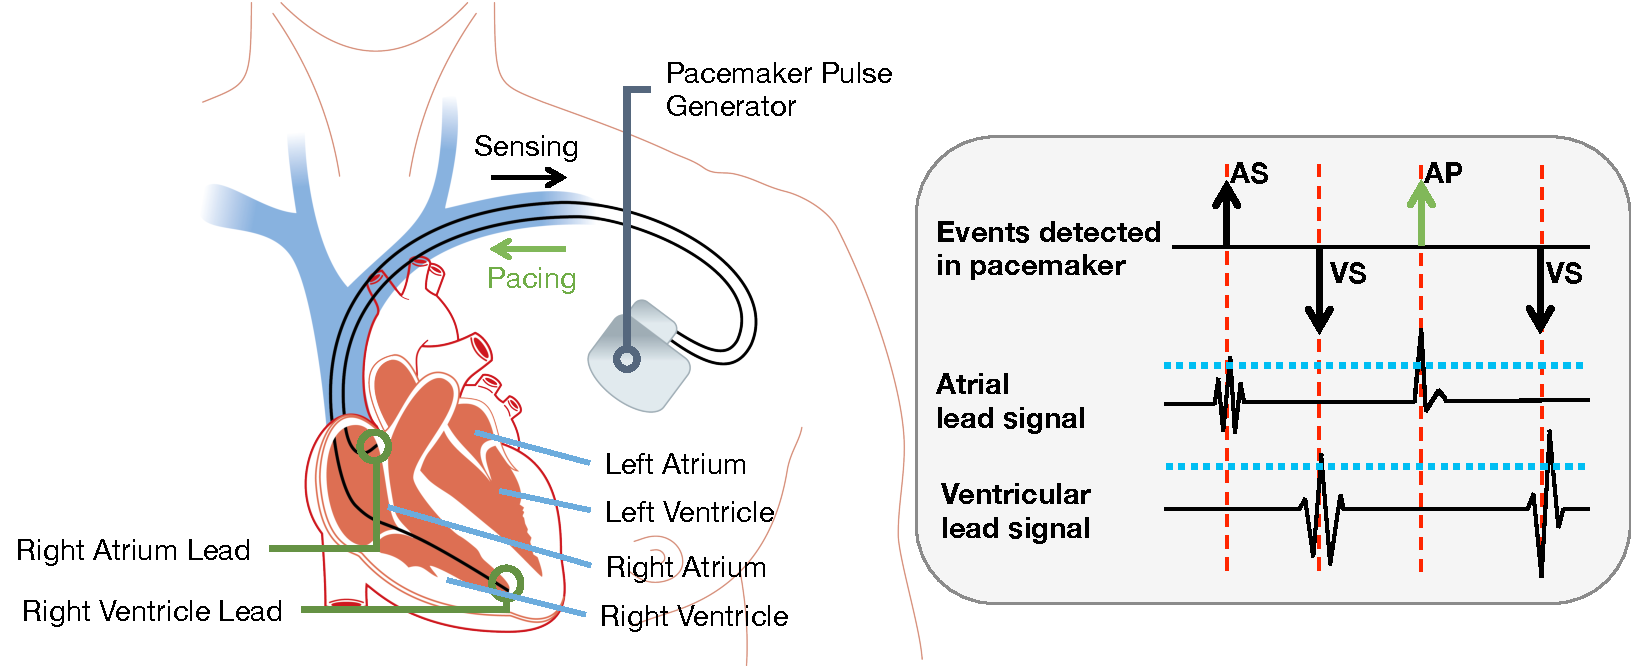
\includegraphics[width=\textwidth]{figs/fig1pacemaker.pdf}
	\caption{\small Pacemaker operating in a closed-loop with the heart. The leads sense cardiac electrophysiological activity from inside the heart tissue (AS/VS = Atrial/Ventricular Sense event) and actuate the heart (AP/VP = Atrial/Ventricular Pacing event} to maintain a desired heart rate.
	\label{fig:pacemaker}
\end{figure}

Open-loop devices are operated by professionals to ensure the safety of the patient.
Closed-loop devices require very little physician intervention after the discharge visit, and hence permit a better lifestyle.
Because they are constantly monitoring the physiological variables, they permit a more timely delivery of therapy. 
The complex run-time diagnoses needed for closed loop performance, and the intricate therapy delivered, has driven most diagnosis and therapy functions into software.
This software is life-critical and verification methods should provide a high confidence in its correctness.

Validating the safety and efficacy of closed-loop software, by definition, requires that the device be connected to the organ(s) it is affecting. 
For example, in the case of a pacemaker, that would be the heart of a living patient.
But with the advent of computer models of physiological functions, such as those encompassed by the Physiome project or presented later in this article, the \emph{model-based design (MBD) of closed-loop medical devices} presents efficient complementary approaches that are actively researched in various disciplines of engineering and computer science.
In MBD, the device (or a model thereof) is connected to a \emph{model} of the ``physiological plant" it interacts with.
By high confidence verification we mean that under all possible behaviors of the physiological models (known or unknown), the device will satisfy its safety properties and not adversely affect the organ.

There are two major differences between modeling physiology and modeling man-made systems:
first, physiology is much more complex and less well-understood than man-made systems like cars and airplanes, and spans several scales from the molecular to the entire human body.
Secondly, the variability between humans is significantly larger than that between two cars coming off the assembly line.
Using the cardiac pacemaker as an example of closed-loop device, and the heart as the organ to be modeled, we present several of the challenges and early results in model-based verification.

